In this chapter we define exactly the kind of concepts and objects we want to represent in our simulation tool before making a survey of the existing simulation software. We then motivate our choice.

\section{Problem statement}
Our robot will consist in a a number of servos connected together through frames in addition to a central plate that will contain the electronics. We also plan to use spring-dampers in the legs to better mimic the human movement an, what is more interesting to us, walk in a more energy efficient way.

If we want to simulate it we thus need a tool that supports:\begin{itemize}
\item inertia, to have physically accurate dynamics.
\item joints, to have constraints between objects.
\item collision and friction, to accurately model the interaction of the feet with the ground.
\item spring-dampers.
\item remote control of the simulation. This is a critical requirement as the goal is to use the same code to control the robot in real-life and the model in the simulation. By control code we mean the high-level code that decides which angles the servos should target, amongst other tasks.
\end{itemize}

The servo used in the robot will have several sensors such as accelerometers, rotary position encoders. We want to model them in the simulator since they will be used by the high-level control code and one of our objectives is the ability to test the latter on the simulator as if it was the real robot. 

We will also have cameras on the robot, so the ability to simulate them would be a plus, still in the mindset that the simulator should be able to substitute itself to the real robot.

\section{Barebone physics engines}
The physics engine is the cornerstone of a physics simulation tool. There exist a quantity of them, we present here the most popular ones that have the following features' set:  multi rigid body dynamics, collision detection, joints (hinge, spring-dampers, generic 6DOF).

\begin{enumerate}
\item \textbf{Bullet\footnote{\url{http://bulletphysics.org/wordpress/}}:} As of now, the most popular open source physics engine. Although primarily used in video games it is also used in applications such as Blender, V-Rep or NASA's tensegrity robotics toolkit. 

\item \textbf{Newton\footnote{\url{http://newtondynamics.com/forum/newton.php}}:} Another open source engine, not quite as popular as Bullet and ODE but nevertheless used for commercial games and simulation. 

\item \textbf{ODE\footnote{\url{https://bitbucket.org/odedevs/ode/}}:} Open source, a little older that Bullet. As it was already mature when simulators started to be developed, it is present in a lot of robotics simulation tools (V-Rep, Webots, Gazebo...). It was also designed with games in mind but was influenced by its success in more serious applications.

\item \textbf{PhysX \& Havok:} Both are proprietary engines used primarily for games. They won't be further discussed because their focus is on speed rather than accurateness and as such they cannot be used in a simulation that aims to be realistic, as stated by Erez \textit{et al} in \cite{engines_comparison}.
\end{enumerate}

\section{Simulators}
In this section we will discuss software that provide a higher level interface to the physics engines we presented earlier. Simulators integrate physics engines and add several higher level functionalities on top of them: visualization, modelling, scripting, etc. 
\begin{enumerate}

\item \textbf{Blender\footnote{\url{https://www.blender.org/} [Accessed 21/05/2016]}} is a 3D modelling software suite and as such has integrated the Bullet engine to help make more realistic animations. It features the ability to make Python scripts that use that engine to make games or physics simulations. 

It is open source and cross platform.

\item \textbf{Gazebo\footnote{\url{http://gazebosim.org/} [Accessed 21/05/2016]}} was the official simulator of DARPA's Robotics challenge. It features multiple physics engines (Bullet, Simbody, Dart and ODE), allows custom plugins and uses the SDF format for its models. 

It is open source but binaries are not provided for Windows and OSX.

\item \textbf{V-Rep\footnote{\url{http://www.coppeliarobotics.com/} [Accessed 21/05/2016]}} is another simulator that lets you choose the physics engine(Bullet, ODE, Newton, Vortex) and it also allows custom plugins in the form of LUA scripts. It uses its own format for storing models but can import standard formats(COLLADA, 3ds, etc...).

It is cross-platform and free to use for educational purposes.

\item \textbf{Webots\footnote{\url{https://www.cyberbotics.com/} [Accessed 21/05/2016]}} has virtually the same features as V-Rep.

It is cross platform but not free.

\item \textbf{Matlab} is not a dedicated robotics simulator \textit{per se} but can be used to model the robot analytically and to write simulation code for it. 
\end{enumerate}
%
%\begin{table}[htp]
%\center
%\begin{tabularx}{\textwidth}{@{} l l X X X X @{}}
%\toprule
%\textbf{Simulator} & \textbf{License} & \textbf{Physics engine(s)} & \textbf{Integrated editor} & \textbf{Modelling}\\ 
%\midrule
%Blender & Free & Bullet & Fully fledged & Internal\\ 
%
%V-REP & Free & Bullet, ODE, Newton, Vortex(10s limit) & Limited & Can import .COLLADA\\
%
%Gazebo & Free & Bullet, ODE, Simbody, DART & Limited & SDF format\\
%
%Webots & Proprietary & ODE & None & SDF format\\
%
%Matlab & Proprietary & None & None & Mathematical\\
%\bottomrule
%\end{tabularx}
%\caption{Comparison of simulators}
%\label{table:simulators_comp}
%\end{table}

\section{Tested software}
In this section we try some of the proposals presented previously and give our thoughts on them. We will mainly look at the modelling facilities and the access to the underlying simulation options as all the proposed tools possess the required simulation capabilities and are able to deliver similar looking results.

\subsection{Blender}
Blender is convenient to use because the robot's model can be easily changed inside. Furthermore, the fact that the scripting language is Python make code development faster and the latter's support of TCP sockets allows an external program to control the simulation and the robot inside it. The internals of the physics are obscured and some interesting object properties, such as inertias, are hard to reach. It is also hard to change the simulation parameters making it difficult to obtain stable results when using a higher number of objects and constraints. Furthermore, support for the game engine, the basis of a simulation project, is uncertain, as stated in the development roadmap \cite{blender_roadmap}.

\textbf{Pros:}
\begin{itemize}
\item Easy modelling of the elements.
\item The Python API is well documented.
\end{itemize}

\textbf{Cons:}
\begin{itemize}
\item Bullet's simulation parameters are hidden behind an incomplete interface, making it impossible to modify the timestep or the number of iterations of the LCP solver.
\item Furthermore, the version Blender uses is an old one and lacks many improvements in the handling of constraints.
\item Inertias are approximated by the principal values Ixx, Iyy and Izz.
\end{itemize}

\subsection{Gazebo}
Gazebo is attractive because it has the support of DARPA and handles multiple physics engines. The main drawback lies in the modelling abilities. It does feature an internal modelling tool but it is too limited to be usable. That would not be a problem if it could import models easily but that is not the case: it uses a format called Unified Robot Description format(URDF) which is a xml based storage format. The problem is that the only tool that can export models in that format is Solidworks\footnote{\url{http://www.solidworks.com/}}, a commercial product. The team behind Gazebo seems to be well-aware that this is an issue since as of may 2016 it is focusing on developing an internal model editor.

\textbf{Pros:}
\begin{itemize}
\item Choice of the physics engine.
\item Inertias definable as a matrix.
\item Friction represented in physical values.
\end{itemize}

\textbf{Cons:}
\begin{itemize}
\item Robot model must be in URDF, making it hard to iterate over robot designs as each model would need to be created by hand.
\item Internal model editor prohibitively limited, cannot be used to create a complicated model.
\end{itemize}

\subsection{V-Rep}
V-Rep also has multiple physics engines available and has a user-friendly interface. It also has an internal modelling tool but there is not much use for it since it allows the import of models in the COLLADA format. Moreover, it supports TCP sockets and even provides code for a client thread in the custom application. The options of the physics engines are also pretty accessible and lots of sensor types are natively supported by the simulator.

\textbf{Pros:}
\begin{itemize}
\item Choice of the physics engine.
\item Inertias definable as a matrix.
\item Friction represented in physical values.
\end{itemize}

\textbf{Cons:}
\begin{itemize}
\item Limited internal editor, can hardly be used for modelling.
\end{itemize}

\section{Choice}
\subsection{Simulator}
We make the choice of using a simulator rather than just a physics engine for several reasons:\begin{itemize}
\item The product of this master's thesis is expected to be used by other students next year and they would rather spend as little time as possible learning how to use it. Hence an established simulator rather than an in-house one is preferred.
\item A simulator eliminates the need of developing 3D visualization by ourselves.
\item A simulator already provides much needed features as the import of 3D models or an interface to the settings of the simulations.
\item Most simulators have an already defined API for remote control.
\item By using an existing simulator we can request help from other users.
\end{itemize}

From the simulators we surveyed earlier in this chapter the best overall seems to be \emph{V-Rep}. This choice is further confirmed by Ivaldi \emph{et al.} in \cite{ivaldi2014tools} who shows that V-Rep is one of the highest rated tools amongst roboticists.

\subsection{Physics engine}
Inside V-Rep, we chose \emph{Newton Dynamics} as the physics engine because simple tests showed it to be the most stable with a high number of joints. That choice is further confirmed by Hummel \textit{et al.} in \cite{hummel2012evaluation} where Newton Dynamics is stated to be the best engine when it comes to handling a high number of constraints.

We will be using the options that are shown in \Cref{fig:newton_options}

\begin{figure}[htp]
	\centering
	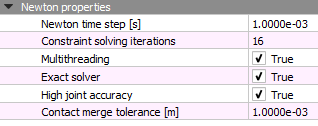
\includegraphics[width=0.6\textwidth]{figures/newton_options}
	\caption{Simulation properties of Newton Dynamics. What is not shown in this figure is the at which the simulator renders the simulation, which is 100Hz. \label{fig:newton_options}}
\end{figure}

\subsection{Modelling software}
Although \emph{Blender} was not chosen as the primary simulation tool for the project, it shall be used as a modelling tool for the robot. The primary reason is that we are already familiar with and we do not need to create elaborate meshes.